%PTRACE CHAPTER 
\chapter{Ptrace}

Like most of the UNIX-like operating systems, Linux supports the \textbf{ptrace} system-call interface. Ptrace provides a means by which a process might observe and control the execution of another process; the first process is referred to as the \textit{tracer} process and the latter as the \textit{tracee} process. Since its introduction in the Linux kernel version 1.0,  ptrace has been mainly employed in implementing debuggers, such as GDB and DBX, where it is used to insert breakpoints into the running program; and for system-call tracing. For example, the command strace exploits ptrace requests to retrieve information regarding the system-calls invoked by a program. 

The ptrace's interface is:
%I use the center environment in order to have the same space 
%between the previous and the next text section.
\begin{center}
\begin{lstlisting}[caption={Synopsis ptrace system call}]
	long ptrace ( enum __ptrace_request request, pid_t pid, void *addr, void *data)
\end{lstlisting}
\end{center}

Ptrace supports numerous different type of actions, for a comprehensive list see  \cite{ptrace}, though the most representative ones are:

\begin{itemize}
\item Attach to, or detach from the process being traced (the tracee), used to install the tracing mechanism.  
\item Read and write the tracee's memory and its status registers.
\item Signal injection and suppression.
\item Resume the execution of the tracee allowing it to continue until 
	  an event of interest occurs ( e.g. a system-call is invoked).
\end{itemize} 

WHEN A PROCESS CAN ATTACH TO ANOTHER PROCESS
The tracer process gains extensive control over the operations of the tracee process. This includes manipulation of its file descriptors, memory, and registers. It can single-step through the tracee's code, observe and intercept system calls and their results. Furthermore, it can manipulate the tracee's signal handlers and both receive and send signals on its behalf. While a process is being traced, all events such as attempting to invoke a system call or receiving a signal are turned into a  \lstinline$SIGCHLD$ \footnote{The communication between the tracee and the tracer is performed using the standard UNIX parent/child signaling over \emph{waitpid} system call}  signals that are delivered to the tracer process. Every time the tracee receives a signal, it is stopped so that the tracer may analyses its status and if necessary changes its execution. 


Although ptrace has been primarily designed for debugging purposes, it offers enough flexibility to be used for different tasks as well. It has been successfully and widely used to implement a \emph{user-space system call interceptor} in [REFERENCES], though it entails numerous limitations. The major disadvantage of the ptrace approach is that the performance may be remarkably reduced in a program which uses intensively system-calls. Several context switches between kernel space and user space are introduced respect to a non-traced execution to support the tracing mechanism. However, an interceptor mechanism can be employed in different contexts and therefore different criteria can be used for choosing it. For example, when performance is not a fundamental requirement such as for debugging, ptrace offers a valid solution. 

One of the most important feature offered by a system-call interceptor is the possibility of retrieving the system call number and its arguments. This may be used in applications for auditing purposes such as strace [ref to strace], where all system calls and their arguments are recorded or sandbox application [references] where each system call is tested against a policy specifying which arguments are allowed and which are not.

Ptrace provides the possibility to retrieve both system call number and its parameters by accessing the status registers and the space memory of the tracee. Accessing the tracee's memory via ptrace is actually rather inefficient as ptrace permits only to pass a small fixed-size block  between the two process. This is one the crucial limitations of ptrace and different techniques have been developed during the recent years to mitigate it. These are presented in the \ref{memory_access} section. 


Another requirement missed by ptrace is to support multi-thread applications. Ptrace actions are specified for single thread via its ID, thus in a multithread application each of its threads must be attached individually. This action if not handled carefully might leave open a temporal window during which some system-calls might not be intercepted. The section  \ref{multi_thread_application} surveys different problems regarding tracing multithread application and provides an effective solution to them.
An important requirement for an application such as a sandbox is the possibility to deny the execution of a system call when it does not satisfy the policy. While other operating system, such Solaris provide a way of aborting a system call, ptrace does not offer any.  In the section \ref{aborting_systemcall} different methods to overcome this shortcoming are introduced.Finally, another requirement missed by ptrace is the possibility to trace only a subset of the system calls provided by the operating system and leave others to be executed without any overhead. This reduces the tracing overhead in several different cases, for example, in a sandbox application  where only the system calls which might affect the security of the operating system should be intercepted. In \cite{Noordende_asecure} all system calls which open or change a file descriptor (open, socket, bind) are intercepted, while those which use it (read, lseek, write) are not. 


Ptrace has been used also for virtualising system calls in \cite{UML_1,goanna, UML_2}. In this case all system-calls invoked by the tracee must be nullified in the host architecture in order to be virtualized; see section \ref{aborting_systemcall}.The ability to write into the tracee's memory allows the tracer to change also the tracee own code segment. This feature has been exploited by specialised programs [reference] to patch running programs in order to avoid  bugs or to fix security lacks. 

Although its limitations and shortcoming ptrace is the standard tracing mechanism used in Linux and Unix-like operating system. This success is due principally to two factors. 
The first is that ptrace provides an easy way to set up the tracing mechanism in user space compared with other approach such us kernel-based tracing mechanism. It can be used without root privilege, provided the tracer has enough privilege to trace the process of interest. Secondly, even though ptrace is not a POSIX system call, it allows for the interception infrastructure to be easily ported between different operating systems.  

The remainder of the chapter introduces how to set up a system call interception using ptrace section \ref{Ptrace_tracing_mechanism} and how to overcome the shortcomings and limitations discussed before. 

%
%How to use Ptrace for intercepting a system call 
%-	Design 
%o	TRACE_ME 
%o	ATTACH 
%	Does the father have enough right to do this?
%	Really bad idea to use root ?? 
%-	How does the tracing mechanism kick off  more or less
%-	How  arguments of a system are accessed 
%-	Why is it important the return value?
%-	System call interposition allows the security kernel model to be extended.
%-	  the monitor is notified each time the target process receives a signal we want to be notified only      for system call trap 
%-	 5     
%-	 6     First part initialization 
%-	 7         atccach, 
%-	 8         there are several trap with multread application       
%-	 9             if they set a paramenter which forbiden tto be traced the ptrace fails 
%-	10                 
%-	11         attach the application musts have the posibility to trace effectivell the target process 
%-	12         this means that it must have the right to do that 
%-	13         the monitor can no be used with root process 
%-	14             a good solution can be to gain root privilege for attach and then release it
\section{Ptrace tracing mechanism}
\label{Ptrace_tracing_mechanism}

Ptrace may be successfully used to build up an effective system call interceptor, ensuring that the tracer process intercepts all system call made by the tracee process and its child processes. This section exposes in details how to implement a system call interceptor using ptrace. 

There are two different ways to install the tracing mechanism. The tracer might invoke the fork system call to create a child process which notifies the kernel its willingness to be traced by calling ptrace with the argument \lstinline$PTRACE_TRACEME$. This request causes the kernel to set a trace flag (\lstinline$PT_TRACED$) in the target process descriptor and stop it by setting its state to non-interruptible sleep. This approach is usually used before the tracing software initiates a new program invoking an exec system call. Alternatively, the monitor process can make a request to the kernel for tracing a running process via ptrace specifying the argument \lstinline$PTRACE_ATTACH$ and the target process pid. In this case, there are three conditions to be checked:
\begin{enumerate}
\item If the privileges of the tracer process allow it to trace the tracee process. Ptrace can attach only to processes that the owner can send signals to (typically only their own processes).
\item If the tracee process is being already traced.
\item If the target process belongs to a set of process that cannot be traced (init and itself).
\end{enumerate}

If all previous controls are satisfied, the monitor process becomes the parent of the traced process and the trace flag is set on its process descriptor. Then, as the previous case, the tracee is put in a non-interruptible sleep state by a \lstinline$SIGSTOP$ signal sent automatically by the kernel. This signal in fact kicks off the tracing mechanism, but it has been seen as possibile source of security issues as a process should not be aware of being traced \cite{ptrace_seize}. In order to overcome this shortcoming the \lstinline$PTRACE_SEIZE$ and \lstinline$PTRACE_INTERUPT$ requests have been introduced in the 3.4 kernel version. \lstinline$PTRACE_SEIZE$ attaches the process specified in the pid to the process that has issued the request. Unlike \lstinline$PTRACE_ATTACH$, \lstinline$PTRACE_SEIZE$ does not stop the process. To stop a process traced using it, an \lstinline$PTRACE_INTERRUPT$ request need to be issued. This cause the stop of the process without sending a SIGSTOP signal, making all the tracing process transparent to the tracee. 
The possibility to attach a running process is particularly useful when a process, which has been created by a different process from the tracer, has to be monitored. A typical example of this situation is when a tracee spawns a new thread. The newly thread must be attached using one of the previous requests as the trace flag is not inherited.  

%% %%% VIRTUAL PARENT `	
It is worth noticing that in both cases the tracer becomes the parent of the tracee process. The \emph{task\_struct} of a Linux process has two fields:
\begin{center}
\begin{lstlisting}[caption={ Parent and real parent fields with task\_struct Linux}]
		struct task_struct *real_parent;	/* real parent process */
		struct task_struct *parent;				/* recipient of SIGCHLD, wait4() reports */
\end{lstlisting}
\end{center}
Usually both field point to the process which has created the current process. When a process is being traced the parent field is modified in order to point to the tracer process which becomes the parent of the child process for most purposes (e.g.,it will receive notification of  child  events  and  appears  in ps(1)  output  as  the  child's parent), while the real parent remains the original one as invoking \lstinline$getpid()$ the pid of the original process is retrieved. In Linux a process has exactly one process father. Consequentially, this limits ptrace to track only one process per time making it a no-efficient mechanism for tracing multithread applications. 
%%%%%%%%%%%%%


When the tracing mechanism has been correctly started, all system calls made by the tracee are intercepted by the tracer. The tracee process is put in a stopped state by the kernel each time it receives a signal or attempts to invoke a system call.  Once the tracee has been stopped, the tracer is notified via a signal \lstinline$SIGCHILD$ and then it is allowed to access the tracee address space.  The tracer may handle this signal either through a wait-family system call or by installing a dedicated handler. 
In the case of system call interceptor, the only relevant notifications are those regarding the attempt of invoking a system call. Precisely, the tracer should be notified twice, at the entry point before the system call is executed and at the exit point before the traced process is resumed. The sequence of events triggered when the traced process invokes a system call is depicted in Figure  \ref{fig:ptrace_systemCall}.

%FIGURE 
\begin{figure}[h]
\centering
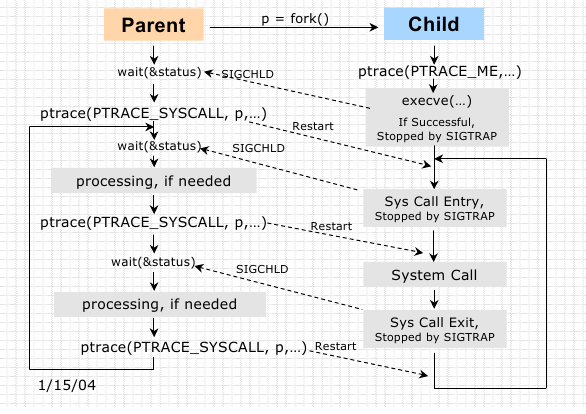
\includegraphics[scale=0.6]{Chapter1/Chapter1Figs/ptrace_systemcall.png} 
\caption{System Call invocation}
\label{fig:ptrace_systemCall}
\end{figure}


The cause of the stop in the tracee can be identified through the status variable returned by the wait primitive or the integer argument in the handler function.  The Linux signal library  provides different macros to easily deal with this signal status variable [ref signal]. The cause that determines the stop of the tracee process can be retrieved as follows:
%Not good we want to identify only system entry adn system exit 
\begin{center}
\begin{lstlisting}[caption={Condition that identifies SIGTRAP signals}]
									WSTOPSIG(status) & (WITSTOPPED(status) == SIGTRAP)
\end{lstlisting}
\end{center}

Unfortunately, the status variable will assume the same value also when a SIGTRAP signal is delivered to the tracee for a different reason from invoking a system call. \\
This ambiguity may be solved in two different ways. Further information about the source of the signal might be retrieved by issuing a ptrace request with \lstinline$PTRACE_GETSIGINFO$.  Although this will introduce a further system call for each SIGTRAP signal delivered to the trace, which in the case of a traced process are the most common.  This performance decrease can be avoided using ptrace with the \lstinline$PTRACE_O_TRACESYSGOOD$ option. This option ensures that when a signal trap is generated because the tracee is trying to make a system call the 7th bit of signal status

\begin{center}
\begin{lstlisting}[caption={Condition that identifies exclusively system call entry and exit}]
									WSTOPSIG(status) & (WITSTOPPED(status)== SIGTRAP | 0x80)
\end{lstlisting}
\end{center}

Now, the tracer can skip all false notifications and analyse only those regarding a system call. 

%PARAMATER ACCESS
One of the most important feature of system call interceptor is the possibility to identify the system call invoked by a process and retrieve all its arguments. The convention adopted in Linux \ref{system_V_abi} for calling a system call is to insert the number of the system call into the EAX register for x32 architecture and in the RAX register in x64, along with its parameters. The maximum number of system call parameters is 6 so the stack is not involved in passing arguments. The table below resumes the role of some registers during a system call invocation for both x32 and x64 architecture, these entire structures can be found in \emph{sys/user.h}. 

\begin{multicols}{2}

\begin{center}
\begin{lstlisting}[caption={Linux structures representing the general purpose registers of x64 CPU}]
/* x64 architecture */				
struct user_regs_struct				
{                                 
  ....                                         
unsigned long int rdi; /* 1th parameter */
unsigned long int rsi; /* 2th parameter */		
unsigned long int rdx; /* 3th parameter */       
unsigned long int rcx; /* 4th parameter */   
unsigned long int r9;  /* 5th parameter */     		
unsigned long int r8;  /* 6th parameter */   
unsigned long int rax;  
/* System Call number */
unsigned long int orig_rax;			   
unsigned long int eflags;            
 ....   
};                                 
\end{lstlisting}
\end{center}

\begin{center}
\begin{lstlisting}[caption={Linux structure representing the general purpose registers of x32 CPU}]
/* x32 architecture */				                                
 struct user_regs_struct
{
  .....
  long int ebx;	 /* 1th parameter */
  long int ecx;  /* 2th parameter */
  long int edx;  /* 3th parameter */
  long int esi;  /* 4th parameter */
  long int edi;  /* 5th parameter */
  long int ebp;  /* 6th parameter */
  long int eax;
  /* System Call number */
  long int orig_eax; 
  long int eflags;
  .... 
};                                 
\end{lstlisting}
\end{center}
\end{multicols}

 
While the tracee process is in stopped, the tracer can retrieve and modify the values of the tracee processor register via PTRACE\_GETREGS/PTRACE\_SETREGS. This methods offers only a way to access to the direct parameters that are conainet in the registers but offers only the possibility to retrieve the indirect parameters whose address is conatained in the resister. In order to retrieve the value of this parameter the tracee memory needs to be accessed. ptrace supports a a request to write into the tracee area adn one request to read from.   

The tracee memory is accessed, before the system call is executed, to retrieve the system call identifier and arguments. This is used in software such as sandbox, for example [systrace, jail, c++] to check whether the system call invocation satisfies the requirements specified in a policy file or for auditing purposes in [systrace]. Furthermore, there is also the possibility to access the tracee memory when the process is stopped after the execution of the system call. This gives a means of analysing the system call return value, which is important for applying post policy rules in a sandbox application [jailer]. Post policy rules are used for those system call where a sensitive value is known only after the call is executed such as accpet, recv. Accessing the memory always introduces an overhead which has to be taken in account when performance is an important aspect of the application. Different approaches for accessing the memory of the tracee process are discussed in detail in \ref{memory_access}. 

Communications between the controller and target take place using repeated calls of ptrace, passing a small fixed-size block of memory between the two (necessitating two context switches per call); this is acutely inefficient when accessing large amounts of the target's memory, as this can only be done in word sized blocks (with a ptrace call for each word).[5] 

retrieve the system call number and the direct arguments  \footnote{ direct argument}. While in order to access to indirect arguments, the space memory of the tracee process need to be accessed. Ptrace offers different type of requests \cite{ptrace} to accomplish this, however all of them are limited in bandwidth to 4 bytes in x32 architecture and 8 bytes in x64.

Ptrace provides for the tracer the ability to fully control the execution of the tracee. The execution of the tracee can be resumed via one of the following ptrace requests:

\begin{description}
\item[PTRACE\_SYSCALL] :
	continues execution until next entry or exit from a system call.
\item[PTRACE\_CONTINUE]:
	 continues execution until the tracee receives a signal.
\item[PTRACE\_SINGLESTEP] :
	continues execution until the next tracee instruction. 
\end{description}

As we are only interested in intercepting a system-calls the execution of a tracee is resumed by calling ptrace with \lstinline$SYS_SYSCALL$ as argument, its execution continuing until the next system call event. 


\section{System call virtualization}
\label{system_call_virtualization}
Virtualization has become increasingly popular and a new demand for Linux is to act as a hypervisor. Different virtualization technologies have been developed to cope this increasing demand, such as instruction emulators QEMU, full or partial hardware emulation.  
System call virtualization is a technique to emulate the execution of a system call made by a process.
Ptrace can be used to set up a system call virtualization mechanism in Linux. This approach has been followed by Jeff Dikk [ two papers]  developing UML whose goals was to run Linux kernel in user space for easing the debugging of kernel.
A system call virtualisation needs a way to nullify system calls so that they would execute in such way as to cause no effects on the host.  However, ptrace did not provide a means of aborting a system call [annulling a system call].  This shortcoming has been fixed introducing the possibility to change to change the actual system call. Annulling a system call can be done by substituting the actual system call with a getpid, which introduces a small overhead due to its execution. \\
When a system call is virtualised, there is no need to intercept the exit point because the system call has been nullified.  This prevents the execution of two context switches between kernel space and user space which yields to a 50\% improvement in the performance.  All these ptrace enhancements have been introduced in the kernel mainline and they can be used by calling ptrace with the parameter SYSEMU [ptrace documentation]. As it has already been said, this prevents the system call to be executed and notifies the tracing parent only at system call entry.  \\
The tracing mechanism can be installed in a similar manner has described in the previous chapter. The only difference is that when the traced software is resumed issuing ptrace with PTRACE\_SYSEMU parameter instead of PTRACE\_SYSCALL.  \\
System call virtualization is implemented by the tracing thread intercepting and redirecting process system calls to the system call handler.  It reads out the system call and its arguments, then annuls this in the host kernel and executes the virtual system call instead. When the emulated system call is finished; the return values are stored in the memory of the traced process.
This process is depicted in the figure. \\
An example of this approach can be found in [GOANA], where ptrace has been used to create a user-level file system development environment.  The bulk of the application consists of a monitor called GOANA which intercepts all system calls made by the traced process. Once the system call has been intercepted this is substituted with a prototype function.  This provides an easy way to test a file system prototype because we do not need to deal with massive body of kernel-level code and  due to the fact it runs on user space the system can be analysed using a powerful debugger such as gdb which would have been impossible to use in kernel mode. \\
The performance is still the main problem of this approach as well.   Even though by using SYSEMU we reduced the context switch between User Space and Kernel space to 2. There is still the necessity   to access the memory at the system call entry point to retrieve its arguments and after the execution of the system call is finished to store the return values. This is a critical part of each monitor process, this problem as in the previous case will be treat in detail in the next section. \\


%%%%%%%%%%%%%%%%%%%%%%%%%%%%%%%%%%%%%%%%%%%%%%%%%%%%%%%%%%%%%%%%%%%%%%%%%  MEMORY ACCESSS %%%%%%%%%%%%%%%%%%%%%%%%%%%%%%%%%%%%%%%%%%%%%%%%%%%%%%%%%%%%%%%%%%%%%%%%%%%%
\section{Memory access}
\label{memory_access}
The tracer process is executed in user mode, it thus is not allowed to write or read the memory space of the tracee process. The tracer needs to read the memory of the tracee process in order to retrieve the contents of the indirect parameters such as strings or pointers.
There are two kinds of arguments direct and indirect, the former is contained in the general purpose register, while the latter is contained in the process memory and its address can be found into registers. The maximum argument number for a system call is six, so they fit in the register and there is no need to access the process stack.Also, the monitor needs to write the target memory address, for instance, when the system call is emulated and the outcome of the computation need to be stored in the traced memory space.

\textbf{Ptrace}\\
One method to access the memory of the tracee process is provided by ptrace. The monitor process may read from the monitor process calling ptrace with PTRACE\_PEEKDATA when the target process is suspended. The writing procedure can be performed in a similar manner by using PTRACE\_POKEDATA. Unfortunately, ptrace transfers only 4 bytes per time, therefore it has to be called many times to read or write a large amount of memory. Every call to ptrace requires a context switch from the monitor to the kernel and back, which decreases its performance since to make it, in fact, not a feasible way with a large amount of data.In order to improve the performance in accessing the traced memory space different approach can be taken.\\

\textbf{Shared Memory}\\
The monitor process has to ensure that the target process can access to the shared memory. In [Jailer] the shared memory is set up using a preload library technique. The preload library uses mmap() to read-only map the memory region in the target’s process space , in addition, it loads some code routine. Another technique presented in [Orchestra] consists of replacing the first system call made by the target process with an appropriate one such as shmget, ipc after making a backup of the values contained in the registers.   This makes the target to run the new syst em call and attaching the shared memory to the target process. After performing this operation, the original system call is restored by using the register values previously saved.  In both cases a small code is injected to the space memory which copies the content of a buffer to another one. When the monitor process needs to access to an indirect arguments, it can retrieve the base address from the registers by using ptrace and then use this routine to copy all the buffer in the share memory. In the Jailer system, the values of registers are modified to point to this memory area for security reasons [See race condition].

\textbf{FIFO}\\
Another approach proposed in [Orchestra] is to use FIFO structures.  FIFO is inter-process communication which allows the monitor process to communicate to the target process by writing to and reading from the FIFO.  The pipe can be created using the system call mkfifo()\cite{Garfinkel03ostia:a} and then it can be managed via I/O system calls usually used to deal with files (in fact the FIFO is a file in the file system). 
The target process can easily open the FIFO by using the FIFO’s name as parameters calling open.  While, if the target process has been spawned by the monitor process, it inheritances the file descriptor corresponding to the FIFO open by monitor process. However, there is still need to use a routine to copy the values from the target process space to the pipe.  Other ipc mechanisms such message queue [jailer] can be used in a similar fashion. \\

\textbf{ Using /proc interface} \\
The proc file system is a pseudo-file system which is used as an interface to kernel data structures. This interface may be used to collect information regarding the execution of a program such as file descriptors, memory layout and so on [ref]. Two files within this hierarchical file system are particular relevant for the purpose of accessing the memory of a traced processed. The first is \lstinline$/proc/pid/maps$ which contains a list of all the memory regions and their access permissions currently mapped in the address space of the process identified by the pid within the path. This feature is used to retrieve the location of shared libraries or shared segment within the address space of a process. It also used to identify whether the process is using a xVSDO mechanism to boost up the process of invoking a system call. The other file of interest is \lstinline$/proc/pid/mem$, it has been introduced to provide an alternative to the ptrace approach discussed before. This file can be used to access the pages of a process's memory via the classic system call  \footnote{The classic system calls used to handle files in Linux are open, lseek, read, write, close} used to deal with files. The two code fragments presents a possible way to implement this approach. Some constrains must be respected by the process that wants to access the memory of another process using this method.
\begin{itemize}
\item  The process that wants to read from or write to \lstinline$/proc/pid/mem$ must trace the execution of the process identified by the pid via ptrace.
\item  The tracee must be in a stopped state.  
\end{itemize} 
If the previous checks are not respected an \lstinline$ESRCH$ error is retrieved. A cautious approach should be taken using this method as the ability of writing to the process's memory might be disable in some kernel versions. This is due to the confusion caused by the introduction of a vulnerability when the writing ability was first activated. The writing function within the kernel carried out a poor permission check which could be exploited by a user to gain root privilege \cite{mem_vul}. However, a recent kernel ( after 3.0) should be bug-free and support the writing function. \\
 
\textbf{Cross memory attach}\\
The space memory of a running process can be also accessed using \emph{cross memory attach}, a new mechanism that has been recently introduced in the Linux kernel
 \ref{cross_memory_attach}. This mechanism is implement by two new system calls \cite{cross memory attach_syscall} that transfer data between the address space of the calling process and the process identified by pid.  The data moves directly between the address spaces of the two processes, without passing through kernel space improving the performance respect to the previous  approach. t has been successfully employed in \cite{mx:icse13} to access the system call's parameters. 
 
For obvious security reasons, there are some restrictions that a process must respect in order to access the memory of another process. In order to perform the copy both process must have the same ownership or the calling process must have the \lstinline$CAP_SYS_PTRACE$ capability. The permission required is exactly the same as that required to perform a ptrace attach to another process. 






\section{Multi thread applications}
\label{multi_thread_application}

 In this chapter, the term multithread process/application refers to an application/process whose threads have been created using the system call \emph{clone} \cite{clone} with the \lstinline$CLONE_THREAD$ flag.
 
Nowadays, most the applications are multithread. For example, a web server usually creates a new thread for each incoming request and let this newly created thread to accomplish it. This family of applications must be taken into account as possible target process for a system call interceptor and this requires a thoroughly analysis. As we already said in the introduction part, one of the most import requirements of a system call interceptor is to provide a means of intercepting all processes spawned by the traced process. Ptrace misses this aspect because it provides a tracing mechanism for single thread [ptrace documentation]; where each thread must be attached individually to the tracer process issuing a request with PTRACE\_ATTACH. Moreover, a child process does not inherit the trace flag from the parent, so it can run untraced until the father attaches to it. These flaws make tracking multithreaded application difficult and error prone [race condition paper], so that some applications [jailer] decided to not support this kind of applications.

Nevertheless, ptrace offers a solution, though it is quite elementary. Setting the option PTRACE\_O\_TRACECLONE [insert a note for other arguments], the tracee will be stopped at the next clone() function and the tracer will start tracing the newly cloned process.  This solution, in fact, is not a feasible way to trace multithread application when performance are important because each time a signal is delivered to a traced thread, all threads in the traced poll enter in a stop state. \\
This introduces an unnecessary latency because the other threads (those that have not received any signal) must wait until the event is processed by the tracer and the entire application is resumed before being able to carry on their tasks. However, in application where performance is not important, for instance debuggers, this represents a valid solution. In fact, this approach is used by GDB.  Another issue related with this approach is that ptrace does not always guarantee that the forked processes are always automatically traced.  Linux allows setting a flag on clone() (CLONE\_UNTRACED)  , which determines whether the child process can be traced or not. However, this can be easily solved noticing that the clone function will be intercepted by the monitor program and it can modify its arguments changing that flag to CLONE\_PTRACE which makes the process traceable.\\ 
The common approach to deal with multithread application is to create a new tracer process [jain and sekar, jailer, orchestra, systrace,strace] for each new tracee process. Unfortunately, this solution raises a race condition which might yield to some system calls to escape from being intercepted. The new monitor is not allowed to trace the newly thread until the parent monitor detaches from it.  When the parent monitors detaches from it the kernel sends a message to the tracee process and allows it to continue its execution.  This leaves a small temporal window within some system calls might escape.  This is critical problem in application such as sandbox, where all system calls must be intercepted for obvious security reason. A completely different approach is taken by strace where this problem is not tackled because a missed system will not comprise the entire application, while solving it will complicate the code, and the temporal window is rather small and the probability of missing a system call or more should be quite low.\\

A possible kernel enhancement, which solves this, would be to notify to the tracer when the newly thread has been created but it is not yet running. This would give the opportunity to safely attach a new tracer to the newly created thread without losing any call. Instead the tracer receives a tracing event only on the child’s subsequent system call.\\
This problem has been addressed successfully in [Orchestra] as follows.  When the tracee process spawns a new thread, automatically it is stopped by the kernel and the monitor start monitoring the newly created thread. At its first system call invocation, the monitor makes a backup of all new tracee process registers and then it substitutes the requested system call with a pause system call and finally lets it continue its execution.  When the new process is resumed, it will enter in a pause state due to the injected system call. While this process is in the sleep state, the monitor is allowed to detach from it and the new monitor can safely attach to it. Once the new monitor has successfully attached, it restores the previous system call so that the execution of the new tracee process can continue. Although this solution works well, it introduces a small time overhead due to the execution of the pause system.  Moreover, a communication between the new monitor and its father is needed to retrieve the backup information regarding the execution context of the new thread in order to restore the previous system call. \\

\section{Aborting a system call}
\label{aborting_systemcall}
Aborting a system call

Having the possibility to abort a system call is an important feature. Let’s consider the following scenario. A large application such as database has been sandboxed for security reason. It is possible that due to the nature of the application and the high number of system call requests, some policy checks fail. When this happen the system call should be nullified, but if this feature is not provided the only solution is to terminate the application even if there is not any real threat.
Unfortunately Linux doesn't provide any means of aborting a system call.  This lack has been one of the main reason because ptrace was not considerate a feasible way to implement a system call interceptor [Janus thesis]. 
Different solutions have been propose [C++ sandbox] and [Goanna], but this problem has been solved by [Uml Guy] who implemented a patch for the Linux kernel. This patch allows the tracer to substitute the invoked system call with another one by inserting a different system call id in the EAX register. Leveraging on the enhancement introduced for UML, the tracee’s system call can be substituted with the low-overhead system call getpid.\\
This technique for aborting a system call raises another problem, which value should be returned? \\
One possibility is EINTR which represent the error code for system call interrupted. However, this is not a good choice because some application may be coded in such a way that, if they receive EINTR error they will retry the system call. If this happens in a loop the application gets stuck and the only way to break that loop is to kill the entire application. A better error code is EPERM, which stands for operation not permitted.\\